\documentclass[
12pt,
a4paper,
bibliography=totocnumbered, %Literaturverzereichnis als Eintrag ins Inhaltsverzeichnis
%twoside, %Zweiseitiger Druck
BCOR=1cm, %Platz zum Lochen
oneside, %Einseitiger Druck
]{scrartcl}

\usepackage{geometry}

\usepackage[default]{fontsetup}
%\usepackage[onehalfspacing]{setspace}

\usepackage[ngerman]{babel}
\usepackage[babel=true,german=quotes]{csquotes}

\usepackage{microtype}
\usepackage{mleftright}
%\newcommand{\Le}{\mleft}
%\newcommand{\Ri}{\mright}
\usepackage[no-script, no-scriptscript, no-inner, no-close]{innerscript}

% Mathepakete (unicode-math ersetzt amssymb, amsfonts etc.)
\usepackage{amsmath,amsthm}
\usepackage{mathtools}
\usepackage{fixdif,derivative}
\usepackage{physics2}
\usephysicsmodule{ab.legacy}

\usepackage{unicode-math}
\setmathfont{NewCMMath-Book}
\setmathfont{NewCMMath-Book}[range=cal, StylisticSet=1]
\setmathfont{NewCMMath-Book}[range=scr]

\usepackage{siunitx}
\sisetup{detect-weight=true, detect-family=true,locale=DE,range-phrase={\,bis\,},list-final-separator ={\,\linebreak[0] \text{und}\,},separate-uncertainty=true,per-mode = symbol-or-fraction}
%\SI[per-mode = fraction]{1}{\meter\per\second} erzwingt auch im Fließtext die Bruchdarstellung.
\DeclareSIUnit\curie{Ci}%Zusätzliche Einheit definieren

\usepackage{tabularx, booktabs, multirow}
\usepackage{array}
\usepackage{enumitem}
\usepackage{float}
\usepackage{graphicx}
\usepackage{xurl}

\usepackage[final]{pdfpages}
\usepackage{framed, color} %Framed: Paket, mittels dessen ein Rahmen um einen Bereich definiert werden kann. Color: Lässt Farbdarstellung in Schrift, Hintergrund etc. zu

\usepackage{scrlayer-scrpage} %Header für die KOMA-script-Klasse

%\usepackage[square,numbers]{natbib}
\usepackage{subfigure} %Mehrere Bilder in einer Figure-Umgebung

\usepackage[bookmarks,colorlinks=true]{hyperref}
\hypersetup{
	colorlinks,
	linktocpage,
	citecolor=black,
	filecolor=black,
	linkcolor=black,
	urlcolor=black,
	pdftitle=X,
	pdfauthor=JM-VS
}

\usepackage[backend=biber, style=chem-angew]{biblatex}
\addbibresource{lit.bib}

\numberwithin{equation}{section} % Die Nummerierung von Gleichungen bekommt die jeweilige Section-Nummer als Präfix

\setlength{\parindent}{0pt} %Einrücktiefe von neuen Absätzen
\setlength{\parskip}{6pt} %Abstand von Absätzen

\pagestyle{scrheadings}%Kopf und Fußzeilen
\ohead{\textbf{\GRUPPENNR\ - \VERSUCHSNR}} %Header oben links auf linker Seite (ungerade Seitenzahl) und oben rechts auf rechter Seite (gerade Seitenzahl), beinhaltet gruppennummer und Versuchskürzel. Im Fall eine einseitigen Dokuments: Header oben rechts
\ihead{\VerfasserEINS\;\&\;\VerfasserZWEI} %Header oben rechts auf linker Seite und oben links auf rechter Seite. Beinhaltet die Namen der Verfasser. Im Fall eine einseitigen Dokuments: Header oben links!
\ofoot{\thepage} %Footer unten links auf linker und unten rechts auf rechter Seite, enthält die jeweilige Seitenzahl. Im Fall eines einseitigen Elements: Footer unten rechts!
\cfoot{\empty} %Mittig unten im Footer soll nichts eingetragen werden
\ifoot{\empty} %Footer unten rechts auf linker und unten links auf rechter Seite. Hier ebenfalls leer.

\newcommand{\tz}{T_{\text{II}}}
\newcommand{\ts}{T_{\text{S}}}
\newcommand{\tgl}{T_{\text{gl}}}
\newcommand{\tgeg}{T_{\text{geg}}}
\newcommand{\omz}{\omega_{\text{II}}}
\newcommand{\omgl}{\omega_{\text{gl}}}
\newcommand{\omgeg}{\omega_{\text{geg}}}
\newcommand{\kB}{k_{\text{B}}}

% Hier können die individuellen Anpassungen vorgenommen werden, die sich auf das Titelblatt und die Kopfzeilen auswirken.

\newcommand{\VERSUCHSDATUM}{29.09.2025}
\newcommand{\PROTOKOLLDATUM}{\today}

\newcommand{\VerfasserEINS}{Julian Molt}
\newcommand{\MatNoEINS}{3803097}
\newcommand{\StudiengangEINS}{Physik}

\newcommand{\VerfasserZWEI}{Valentin Stopper}
\newcommand{\MatNoZWEI}{3774391}
\newcommand{\StudiengangZWEI}{Physik}

\newcommand{\BETREUER}{Julian Vollmer}
\newcommand{\GRUPPENNR}{A-016}

\newcommand{\VERSUCHSNR}{E24}
\newcommand{\VERSUCHSNAME}{Halbleiterdioden}

\newcommand{\lh}{\ell_{\mathrm{H}}}
\newcommand{\ls}{\ell_{\mathrm{S}}}


\begin{document}

\thispagestyle{empty}

\begin{titlepage}

	\begin{center}
		\Huge{\textbf{\VERSUCHSNR\ -- \VERSUCHSNAME}}\\
		\vspace{10mm}
		\Large{Protokoll zum Versuch des Physikalischen Praktikums I von \\ \textbf{\VerfasserEINS\;\& \VerfasserZWEI}}\\
		\vspace{10mm}
		\Large{Universität Stuttgart}\\
	\end{center}
	\vspace{1cm}
	\begin{center}
		\begin{tabular}{ll}
			\large{Verfasser:}		& \large{\VerfasserEINS\;(\StudiengangEINS),} \\
			& \large{\MatNoEINS} \\
			\vspace{0cm}\\
			& \large{\VerfasserZWEI\;(\StudiengangZWEI),} \\
			& \large{\MatNoZWEI} \\
			\vspace{0cm}\\
			\large{Gruppennummer:}	& \large{\GRUPPENNR} \\
			\vspace{0cm}\\
			\large{Versuchsdatum:}	& \large{\VERSUCHSDATUM} \\
			\vspace{0cm}\\
			\large{Betreuerin:}		& \large{\BETREUER}
		\end{tabular}
	\end{center}
	\vspace{15mm}

	\begin{center}
		Stuttgart, den \PROTOKOLLDATUM
	\end{center}

\end{titlepage}

\thispagestyle{empty}

\tableofcontents

\clearpage %Neue Seite, davor werden alle noch ausstehenden Grafiken/Tabellen platziert.

\renewcommand{\thepage}{\arabic{page}}
\setcounter{page}{1}


% Die erste eckige Klammer ist optional, die darin angegebene Bezeichnung steht im Inhaltsverzeichnis anstelle des hinteren (längeren) Namens.
\section[Versuchsziel]{Versuchsziel und Versuchsmethode}

In diesem Versuch werden Halbleiterdioden untersucht. Dazu werden die Kennlinien einer Silizium- und Germaniumdiode, einer Z-Diode und von zwei LEDs aufgezeichnet. Für die Z-Diode und die LEDs geschieht dies mithilfe eines Oszilloskops.

\section{Grundlagen}

Elektronen können in einem Atom diskrete Energieniveaus einnehmen. Nähern sich Atome einander an werden die Energieniveaus zu mehreren naheliegenden Energieniveaus aufgespalten. Innerhalb eines Einkristalls, mit vielen wechselwirkenden Atomen, kommt es zu vielen Aufspaltungen, weshalb naheliegende Energieniveaus zu Bändern zusammengefasst werden. Diese Bänder können von Elektronen besetzt werden. Das höchste vollbesetzte Band heißt Valenzband. Das energetisch über dem Valenzband liegende Band heißt Leitungsband. Ein Kristall ist dann leitend, wenn er ein teilweise besetztes Band hat, da die Elektronen nur dann ein höheres Energieniveau einnehmen können, um Energie zu übertragen.

Als Bandlücke wird der Energiebereich zwischen Valenz- und Leitungsband bezeichnet. Die Energieniveaus innerhalb der Bandlücke können von Elektronen nicht eingenommen werden. Bei Isolatoren ist das Leitungsband unbesetzt und die Bandlücke groß, weshalb keine Elektronen einfach ins Leitungsband gelangen. Bei Halbleitern ist die Bandlücke kleiner, wodurch Elektronen unter moderater Energiezufuhr, wie bspw. Wärme oder Licht, ins Leitungsband gelangen können.

Alternativ kann die Leitfähigkeit eines Halbleiters auch durch Dotierung verbessert werden. Bei der p-Dotierung werden in den Halbleiterkristall Atome niedrigerer Wertigkeit, also mit weniger Valenzelektronen, als die Atome des Halbleiterkristalls hat, eingebracht. Diese Fremdatome heißen Akzeptoren. Bei der n-Dotierung werden Atome höherer Wertigkeit eingebracht und sie heißen Donatoren. Dadurch entstehen freie Elektronen, bzw. Elektronenfehlstellen, die Strom leiten können.
Werden ein p- und ein n-dotierter Halbleiter zusammengeführt, entsteht ein pn-Übergang. Durch den pn-Übergang bewegen sich Elektronen und Fehlstellen aufeinander zu und rekombinieren. Dadurch bleiben auf der p-dotierten Seite die negativ geladenen Atomrümpfe der Akzeptoren und auf der n-dotierten Seite die positiv geladenen Rümpfe der Donatoren übrig. Dadurch entsteht ein elektrisches Feld, was die Diffusion beider Ladungsträger bremst. Schlussendlich stellt sich ein Gleichgewicht ein, sodass kein Ladungstransport mehr stattfindet. Diesen mittlere Bereich des pn-Übergangs, in dem das Feld wirkt, nennt man Raumladungszone oder Sperrschicht.

Wird eine Spannung angelegt, mit negativem Pol an der n-dotierten Seite und positivem Pol an p-dotierten Seite, wird das elektrische Feld abgebaut und schließlich fließt Strom in Durchlassrichtung, unter ständiger Rekombination, bei der Energie frei wird. Polt man die angelegte Spannung um, sperrt die Diode und es fließt ausschließlich ein geringer Sperrstrom \(I_{\text{S}}\), welcher nicht durch Rekombination hervorgeht, sondern durch thermisch aktivierte Elektronen. Für  ideale pn-Übergänge von Dioden gilt die  Shockley'sche Beziehung
\begin{equation}
I=I_{\text{S}} \cdot \mleft[\exp\mleft( \frac{eU}{\kB T}\mright)-1 \mright]\,.
\end{equation}
Dabei steht \(e\) für die Elementarladung, \(\kB\) für die Boltzmankonstante, \(U\) für die Spannung und \(T\) für die Temperatur.
Bei einer sehr hohen Sperrspannung kann es zu einem hohen Sperrstrom, abweichend von der Shockley'schen Beziehung kommen. Der Hintergrund dafür ist einerseits der Zenereffekt, bei dem durch die Sperrspannung das Valenzband des p-dotierten Halbleiters und das Leitungsband des n-dotierten Halbleiters auf dasselbe Energieniveau gehoben werden. Dadurch können Elektronen vom Valenz- direkt ins Leitungsband gelangen und ein Stromfluss wird möglich. Bei Zenerdioden handelt es sich um stark dotierte Siliziumdioden, die sich genau diesen Effekt zunutze machen.

Andererseits kann es zum Lawineneffekt kommen, bei dem freie, beschleunigte Elektronen andere Elektronen so schnell aus dem Gitter stoßen, dass keine Rekombination stattfinden kann. Diese stoßen wiederum gegen andere Elektronen, was einen schlagartigen Stromanstieg zur Folge hat.
LEDs sind Dioden, bei denen Lichtquanten unter Rekombination entstehen.

Die elektrische Leitfähigkeit \(\sigma\) ist gegeben durch
\begin{equation}
	\sigma = \frac{1}{\rho}
\end{equation}
mit dem spezifischen Widerstand \(\rho\).
Der Widerstand \(R\) ist gegeben als
\begin{equation}
	R = \rho \cdot \frac{\ell}{A} \,,
\end{equation}
wobei \(\ell\) die Länge des Leiters und \(A\) dessen Querschnitt sind. Daraus folgt für die elektrische Leitfähigkeit
\begin{equation}\label{eq:Leitfähigkeit}
	\sigma = \frac{\ell}{RA} \,.
\end{equation}
%\begin{figure}[H]
%	\centering{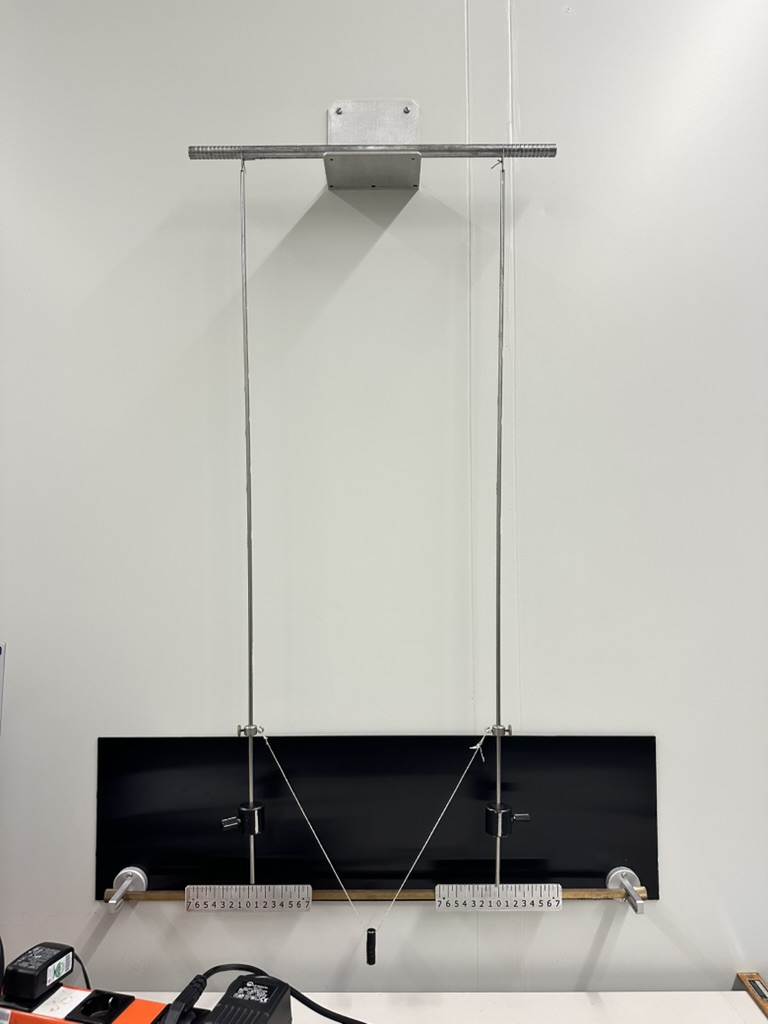
\includegraphics[width=0.4\textwidth]{Aufbau}}
%	\caption{Aufbau der Pendel, die hier bei \(\lh = \qty{70}{\centi\meter}\) gekoppelt sind.}
%	\label{fig:aufbau}
%\end{figure}

\section[Messprinzip]{Messprinzip mit Abbild und Versuchsablauf}

\begin{figure}[H]
	\centering{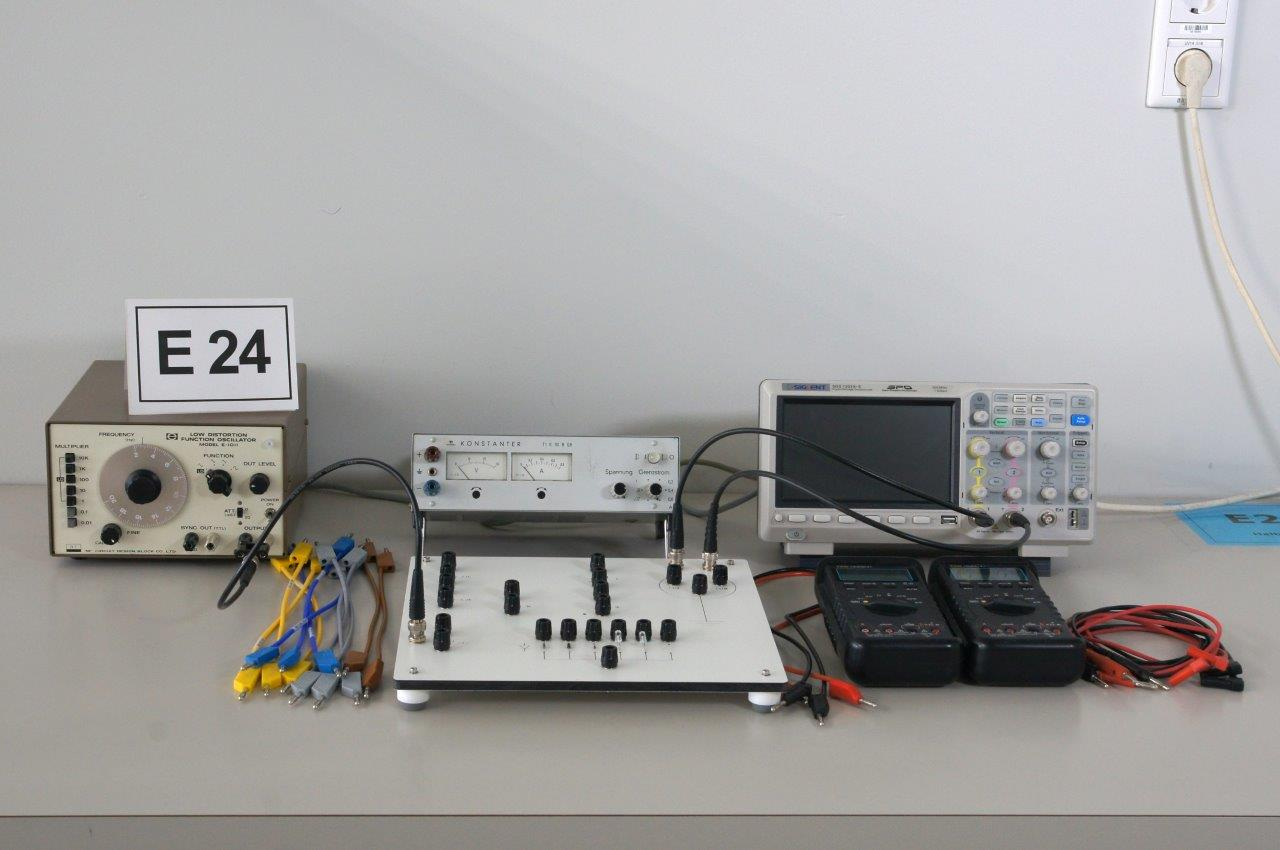
\includegraphics[width=0.9\textwidth]{E24versuchsaufbau.jpg}}
	\caption{Versuchsaufbau mit Gleich- und Wechselspannungsquelle, Digitalmultimetern und Oszilloskop \cite{Quelle}.}
	\label{fig:Aufbau}
\end{figure}
Auf dem Steckbrett sind die verschiedenen abgreifbaren Dioden.
Im ersten Versuchsteil wird die Gleichstromspannungsquelle genutzt um die Dioden erst in Fluss- und dann in Sperrrichtung zu betreiben. Die Messwerte werden hier mit den zwei Multimetern bestimmt.

In den restlichen Versuchsteilen wird der Wellengenerator genutzt, um eine Wechselspannung zu erzeugen. Hier werden die Messdaten mit dem Oszilloskop erhoben.


\section{Messwerte}

\begin{table}[H]
	\centering % damit die Tabelle trotzdem mittig steht
	\caption{Gemessene Spannung und Strom der Germanium-Diode in Durchlassrichtung.\label{tbl:GeDiode}}
	\begin{tabular}{ll}
		\toprule
		Spannung in \si{\milli\volt} & Strom in \si{\micro\ampere} \\
		\midrule
		\num{22,7}  & \num{0,06}  \\
		\num{100,2} & \num{11,9}  \\
		\num{152,0} & \num{55,5}  \\
		\num{199,3} & \num{182,3} \\
		\num{210,2} & \num{234,4} \\
		\num{220,2} & \num{292,3} \\
		\num{230,1} & \num{360}   \\
		\num{250,6} & \num{550}   \\
		\num{270,3} & \num{810}   \\
		\num{283,6} & \num{1050}  \\
		\num{320,3} & \num{1980}  \\
		\num{346,0} & \num{2990}  \\
		\num{366,0} & \num{4020}  \\
		\num{383,0} & \num{5020}  \\
		\num{397,0} & \num{5990}  \\
		\num{410,0} & \num{6990}  \\
		\num{422,0} & \num{8000}  \\
		\bottomrule
	\end{tabular}
\end{table}

\begin{table}[H]
	\centering % damit die Tabelle trotzdem mittig steht
	\caption{Gemessene Spannung und Strom der Silizium-Diode in Durchlassrichtung.\label{tbl:SiDiode}}
	\begin{tabular}{ll}
		\toprule
		Spannung in \si{\milli\volt} & Strom in \si{\micro\ampere} \\
		\midrule
		\num{99,4}  & \num{0,2} \\
		\num{155,2}  & \num{0,2} \\
		\num{208,2}  & \num{0,1} \\
		\num{304,6}  & \num{1}  \\
		\num{400}  & \num{11,8}  \\
		\num{452}  & \num{47,3}  \\
		\num{500}  & \num{149,3} \\
		\num{520}  & \num{238,9} \\
		\num{539}  & \num{355} \\
		\num{580}  & \num{820} \\
		\num{598}  & \num{1220} \\
		\num{623}  & \num{2020} \\
		\num{641}  & \num{2970} \\
		\num{655}  & \num{3980} \\
		\num{666}  & \num{5050} \\
		\num{674}  & \num{6020} \\
		\num{681}  & \num{7020} \\
		\num{687}  & \num{8010} \\
		\bottomrule
	\end{tabular}
\end{table}

\begin{table}[H]
	\centering % damit die Tabelle trotzdem mittig steht
	\caption{Gemessene Spannung und Strom der Silizium-Diode.\label{tbl:TempSi}}
	\begin{tabular}{lrr}
		\toprule
		Temperatur & Spannung in \si{\milli\volt} & Strom in \si{\micro\volt} \\
		\midrule
		\enquote{kalt} & \num{517} & \num{199,6} \\
		\enquote{warm} & \num{510} & \num{204,6}\\
		\bottomrule
	\end{tabular}
\end{table}

\begin{table}[H]
	\centering % damit die Tabelle trotzdem mittig steht
	\caption{Gemessene Spannung und Strom der Silizium-Diode.\label{tbl:TempGe}}
	\begin{tabular}{lrr}
		\toprule
		Temperatur & Spannung in \si{\milli\volt} & Strom in \si{\micro\volt} \\
		\midrule
		\enquote{kalt} & \num{201,9} & \num{200,4} \\
		\enquote{warm} & \num{191,5} & \num{207,4} \\
		\bottomrule
	\end{tabular}
\end{table}

\begin{table}[H]
	\centering % damit die Tabelle trotzdem mittig steht
	\caption{Gemessene Spannung und Strom der Silizium-Diode in Sperrrichtung.\label{tbl:SiSperr}}
	\begin{tabular}{ll}
		\toprule
		Spannung in \si{\milli\volt} & Strom in \si{\micro\volt} \\
		\midrule
		\num{0,517} & \num{0,2} \\
		\num{1,061} & \num{0,3} \\
		\num{2,032} & \num{0,4} \\
		\num{3,220} & \num{0,5} \\
		\num{4,060} & \num{0,6} \\
		\num{5,120} & \num{0,7} \\
		\num{6,070} & \num{0,8} \\
		\num{7,060} & \num{0,9} \\
		\num{7,770} & \num{1,0} \\
		\bottomrule
	\end{tabular}
\end{table}

\begin{table}[H]
	\centering % damit die Tabelle trotzdem mittig steht
	\caption{Gemessene Spannung und Strom der Germanium-Diode in Sperrrichtung.\label{tbl:GeSperr}}
	\begin{tabular}{ll}
		\toprule
		Spannung in \si{\milli\volt} & Strom in \si{\micro\volt} \\
		\midrule
		\num{0,518} & \num{0,7} \\
		\num{1,014} & \num{0,8} \\
		\num{1,527} & \num{0,9} \\
		\num{2,996} & \num{1,1} \\
		\num{4,050} & \num{1,2} \\
		\num{5,200} & \num{1,4} \\
		\num{6,000} & \num{1,5} \\
		\num{6,810} & \num{1,6} \\
		\num{7,510} & \num{1,7} \\
		\num{7,770} & \num{1,0} \\
		\bottomrule
	\end{tabular}
\end{table}

\section{Auswertung}

Die Kennlinie für den Durchlassbereich der Silizium- und Germanium-Diode wird mit digitalen Multimetern gemessen. Die aufgenommenen Messpunkte werden dann halblogarithmisch als Durchlasskennlinie aufgetragen. Der graphisch extrapolierte Sperrstrom beträgt für die Silizium-Diode \qty{2,09e-9}{\ampere} und für die Germanium-Diode \qty{3,16e-9}{\ampere}.
\begin{figure}[H]
	\centering{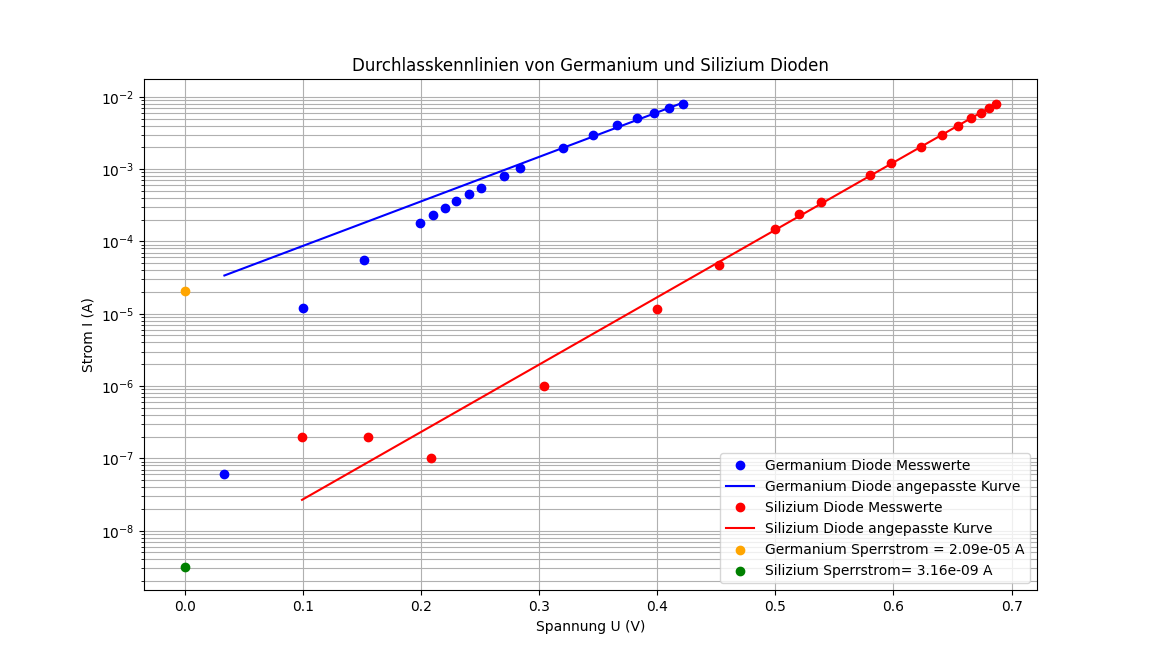
\includegraphics[width=0.9\textwidth]{DurchlasskennlinieSiGe.png}}
	\caption{Sperrkennlinien der Si- und Ge-Dioden.}
	\label{fig:Durchlass}
\end{figure}

Die Leitfähigkeit der kalten Diode beträgt nach \autoref{eq:Leitfähigkeit}
\begin{equation}
	\sigma_{\text{k}} = \frac{\ell}{R_{\text{k}}A}
\end{equation}
und für die Warme
\begin{equation}
	\sigma_{\text{w}} = \frac{\ell}{R_{\text{w}}A} \,.
\end{equation}

Somit ist die prozentuale Änderung der Leitfähigkeit \(\Delta \sigma\) für die Silizium-Diode
\begin{align*}
	\Delta \sigma &= \frac{\sigma_{\text{w}}}{\sigma_{\text{k}}} -1 = \frac{\frac{\ell}{R_{\text{w}}A}}{\frac{\ell}{R_{\text{k}}A}} -1 = \frac{R_{\text{k}}}{R_{\text{w}}} -1 = \frac{\frac{U_{\text{k}}}{I_\text{k}}}{\frac{U_{\text{w}}}{I_{\text{w}}}} -1\\
	&= \frac{\frac{\qty{517e-3}{\volt}}{\qty{199,6e-6}{\ampere}}}{\frac{\qty{510e-3}{\volt}}{\qty{204,6e-6}{\ampere}}} -1 = \frac{\qty{2492,67}{\ohm}}{\qty{2590,18}{\ohm}} -1\\
	&= \qty{-4}{\percent} \,.
\end{align*}
Für die Germanium-Diode ergibt sich eine Änderung von \qty{-8}{\percent}.

Bei Messung der Sperrkennlinien der beiden Dioden muss auch der Fehlerstrom \(I_{\text{err}}\) einberechnet werden. Vorher war dieser zu vernachlässigen, da der Innenwiderstand des Voltmeters sehr hoch ist, der der Diode in Durchlassrichtung aber sehr klein. In Sperrrichtung ist der Widerstand der Diode groß, was bedeutet, dass sich der Strom mehr auf die Diode und das Spannungsmessgerät aufteilt. Er berechnet sich folgendermaßen:
\begin{equation*}
	I_{\text{err}} = \frac{U}{R_{\text{Messgerät}}}
\end{equation*}
Hierbei wird angenommen, dass der Widerstand des Amperemeters vernachlässigbar klein ist und somit die Spannung, die vom Voltmeter angezeigt wird, die ist, die über die Diode abfällt.

Der Fehlerstrom muss vom gemessenen Strom des Amperemeters abgezogen werden, wonach die Sperrkennlinien wie sie in \autoref{fig:Sperrkennlinien} zu sehen sind, zustande kommen.
\begin{figure}[H]
	\centering{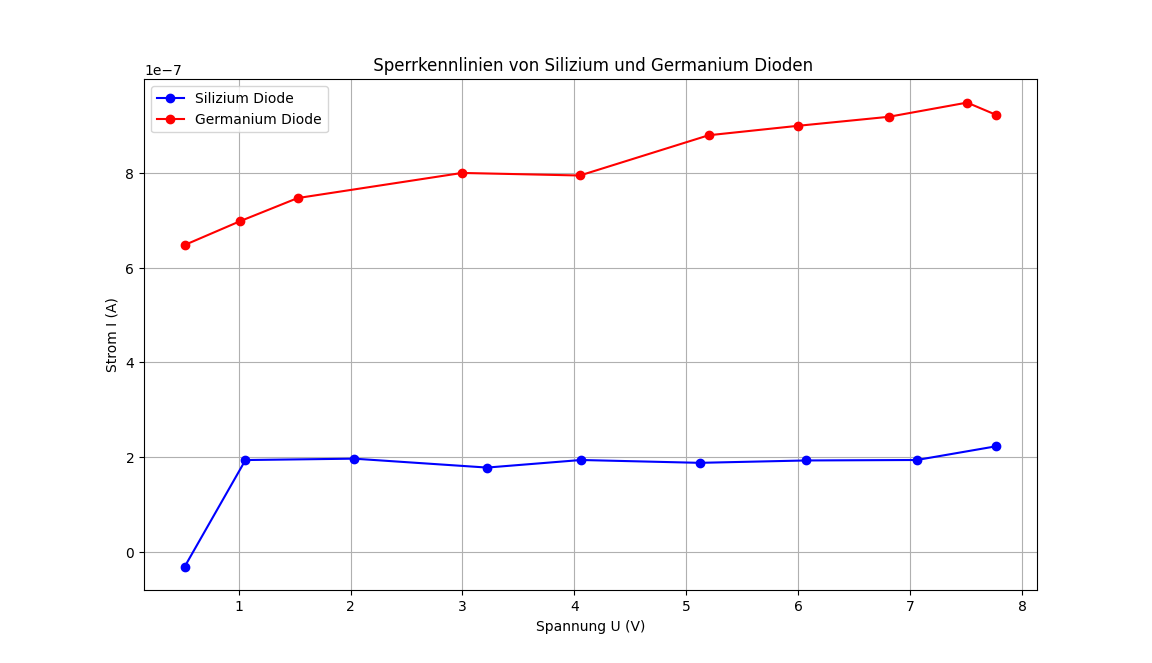
\includegraphics[width=0.9\textwidth]{SperrstromSiGe.png}}
	\caption{Sperrkennlinien der Si- und Ge-Dioden.}
	\label{fig:Sperrkennlinien}
\end{figure}

Die Kennlinie der Z-Diode wird mit einem Oszilloskop gemessen und kann in einem linearen Diagramm dargestellt werden.
\begin{figure}[H]
	\centering{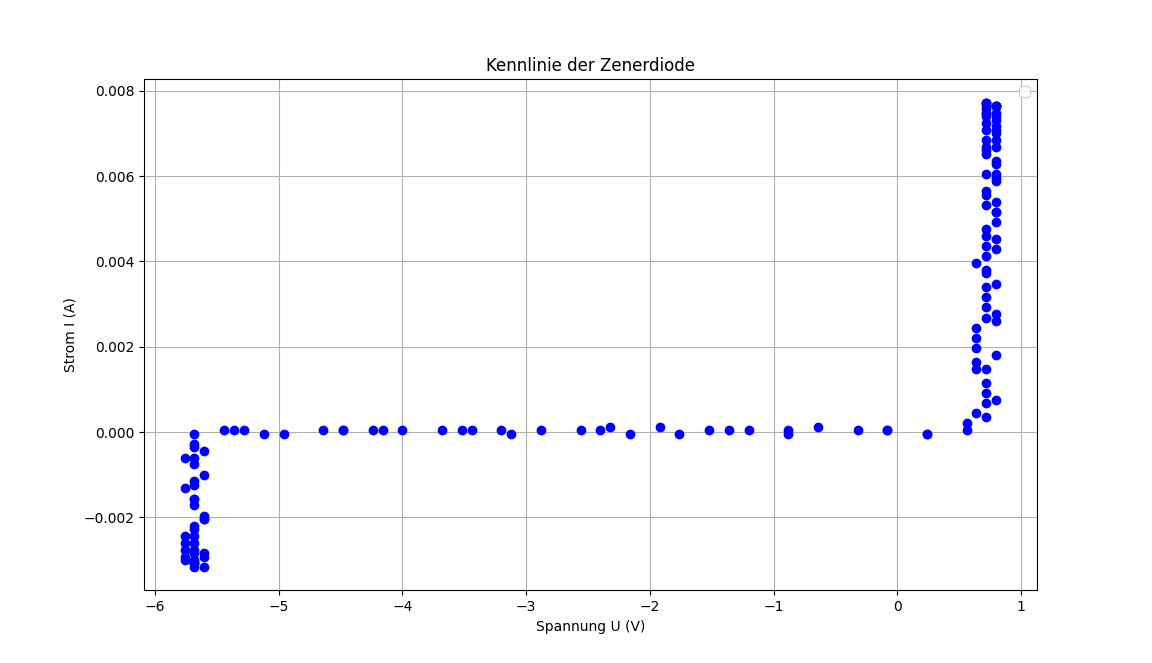
\includegraphics[width=0.9\textwidth]{KennlinieZ.png}}
	\caption{Kennlinie der Z-Diode.}
	\label{fig:KennlinieZ}
\end{figure}

In Flussrichtung verhält die Zenerdiode sich wie eine normale Diode, weshalb sie den klassischen exponentiellen Anstieg der Stromstärke, ab einer Spannungsschwelle zeigt. In Sperrrichtung fließt erst der Sperrstrom, bis auch dann wieder ein exponentieller Anstieg beobachtbar ist. Dieser Entsteht, da die Zenerdiode den Zenereffekt nutzt, um ab einer gewissen Sperrspannung wieder leitend zu sein.


Die Kennlinien einer roten und blauen LED werden ebenfalls mit einem Oszilloskop aufgenommen führen auf die folgenden Kennlinien.
\begin{figure}[H]
	\centering{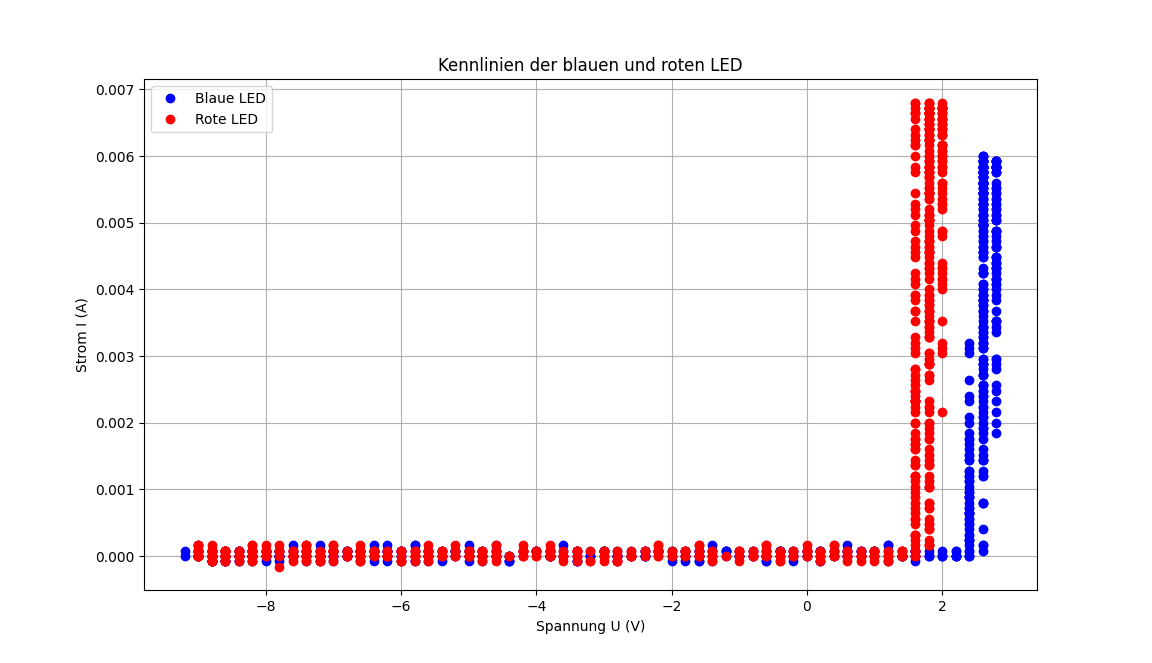
\includegraphics[width=0.9\textwidth]{KennlinieLED.png}}
	\caption{Kennlinie einer roten und einer blauen LED.}
	\label{fig:KennlinieLED}
\end{figure}

Es ist deutlich zu erkennen, dass die rote LED eine niedrigere Schwellenspannung besitz, als die Blaue. Das liegt am unterschiedlichen Aufbaue beider Dioden. Bei beiden Dioden wird die Lichtemission dadurch ausgelöst, dass, sobald die LED in Durchlassrichtung geschaltet ist, Elektronen im Leiterband von der n-dotierten Seite auf die p-dotierte Seite gelangen und dort unter Emission von Photonen mit den Deffektelektronen rekombinieren.

Ein Elektron hat die Energie
\begin{equation*}
	E = e \cdot U \,.
\end{equation*}
Als Näherung kann man annehmen dass diese Energie vollständig als Licht emittiert wird. Die Energie von Licht mit der Wellenlänge \(\lambda\) ist
\begin{equation*}
	E_{\text{L}} = \frac{hc}{\lambda}
\end{equation*}
mit dem Planck'schen Wirkungsquantum \(h\) und der Lichtgeschwindigkeit \(c\).
Dann lautet die Relation zwischen angelegter Spannung und Wellenlänge
\begin{equation*}
	U = \frac{hc}{e\lambda}
\end{equation*}
%\section{Fehlerrechnung}
Für rotes Licht wird eine Wellenlänge von \(\lambda_{\text{R}} = \qty{700}{\nano\meter}\) angenommen, was zu einer Schwellenspannung von
\begin{align*}
	U &= \frac{hc}{e\lambda_{\text{R}}} = \frac{\qty{6,62607015e-34}{\joule\second} \cdot \qty{299792458}{\meter\per\second}}{\qty{1,602176634e-19}{\coulomb} \cdot \qty{700e-9}{\meter}}\\
	&\approx \qty{1,77}{\volt}
\end{align*}
führt.
%Diese befindet sich am oberen Ende des sichtbaren elektromagnetischen Spektrums und entspricht folgerichtig rotem Licht. Für die blaue Diode ergibt sich mit \(U_{\text{Schwelle}} = \qty{2,3}{\volt}\) eine Wellenlänge von \(\lambda \approx \qty{539}{\nano\meter}\), was deutlich niedriger ist und sich im Bereich von blauem und grünem Licht befindet. Damit sind die Korrelationen zwischen Schwellenspannung und Wellenläge der LED bestätigt.
Für blaues Licht wird eine Wellenlänge von \(\lambda_{\text{B}} = \qty{450}{\nano\meter}\) angenommen woraus sich eine Schwellenspannung von \(U \approx \qty{2,76}{\volt}\) ergibt.

Bei der roten LED wird eine Schwellspannung von \qty{1,54}{\volt} und bei der Blauen \qty{2,3}{\volt} gemessen. Für diese einfachste Näherung lässt sich unter den berechneten und experimentell bestimmten Werten eine qualitative Übereinstimmung schließen.

Die abgegebenen Leistung \(P_4\) in den Widerstand \(R_4\), sowie die die Eingangsleistung \(P_2\) werden durch die Effektivwerte der Spannung und des Stromes bestimmt. Dafür gilt
\begin{equation*}
	P_{\text{eff}} = U_{\text{eff}} \cdot I_{\text{eff}} = \frac{\hat{U}}{\sqrt{2}} \cdot \frac{\hat{I}}{\sqrt{2}} = \frac{1}{2} \cdot \hat{U} \cdot \hat{I} \,,
\end{equation*}
wobei \(\hat{U}\) und \(\hat{I}\) der Scheitelwert der Wechselspannung bzw. des Wechselstromes sind.
Für die Eingangsleistung mit der Silizium-Diode ergibt sich zum Beispiel
\begin{equation*}
	P_2 = \frac{(\qty{8,33}{\volt})^2}{2 \cdot \qty{1}{\kilo\ohm}} = \qty{34,69}{\milli\watt} \,.
\end{equation*}
In \autoref{tbl:POWER} sind alle Eingangsleistungen, sowie die Leistungen über \(R_4\) dargestellt.
\begin{table}[H]
	\caption{Eingangsleistungen und Leistungen über Widerstand \(R_4\) \label{tbl:POWER}}
	\begin{tabular*}{\textwidth}{@{\extracolsep{\fill}}@{\hspace{5pt}}lrr@{\hspace{5pt}}}
		\toprule
		Diode & \(P_2\) in \si{\milli\watt} & \(P_4\) in \si{\milli\watt} \\
		\midrule
		Silizium & \num{34,69} & \num{29,18} \\
		Germanium & \num{34,44} & \num{30,81} \\
		LED (Blau) & \num{34,36} & \num{15,96} \\
		LED (Rot) & \num{34,36} & \num{21,51} \\
		\bottomrule
	\end{tabular*}
\end{table}

Die mittlere Spannung \(\hat{U}\) über eine Halbwelle kann durch das Integral
\begin{equation*}
	\hat{U} = \frac{1}{t_2 - t_1} \cdot \int\limits_{t_1}^{t_2} U(t) \d t
\end{equation*}
bestimmt werden. Dies wurde numerisch in Python durchgeführt, da das Oszilloskop keine stetige Funktion liefert, sondern Daten in Form von Datenpunkten.
Die Ergebnisse sind in \autoref{tbl:middleU} tabelliert.
\begin{table}[H]
	\caption{Eingangsleistungen und Leistungen über Widerstand \(R_4\) \label{tbl:middleU}}
	\begin{tabular*}{\textwidth}{@{\extracolsep{\fill}}@{\hspace{5pt}}lrr@{\hspace{5pt}}}
		\toprule
		Diode & \(\hat{U}_4\) in \si{\volt} & \(\hat{U}_2\) in \si{\volt} \\
		\midrule
		Silizium & \num{5,00} & \num{5,50} \\
		Germanium & \num{5,24} & \num{5,55} \\
		LED (Blau) & \num{3,15} & \num{5,58} \\
		LED (Rot) & \num{3,91} & \num{5,56} \\
		\bottomrule
	\end{tabular*}
\end{table}

Die Eingangsleistungen, sowie die abfallenden Leistungen können zudem in Diagrammen sichtbar gemacht werden:
\begin{figure}[H]
	\centering{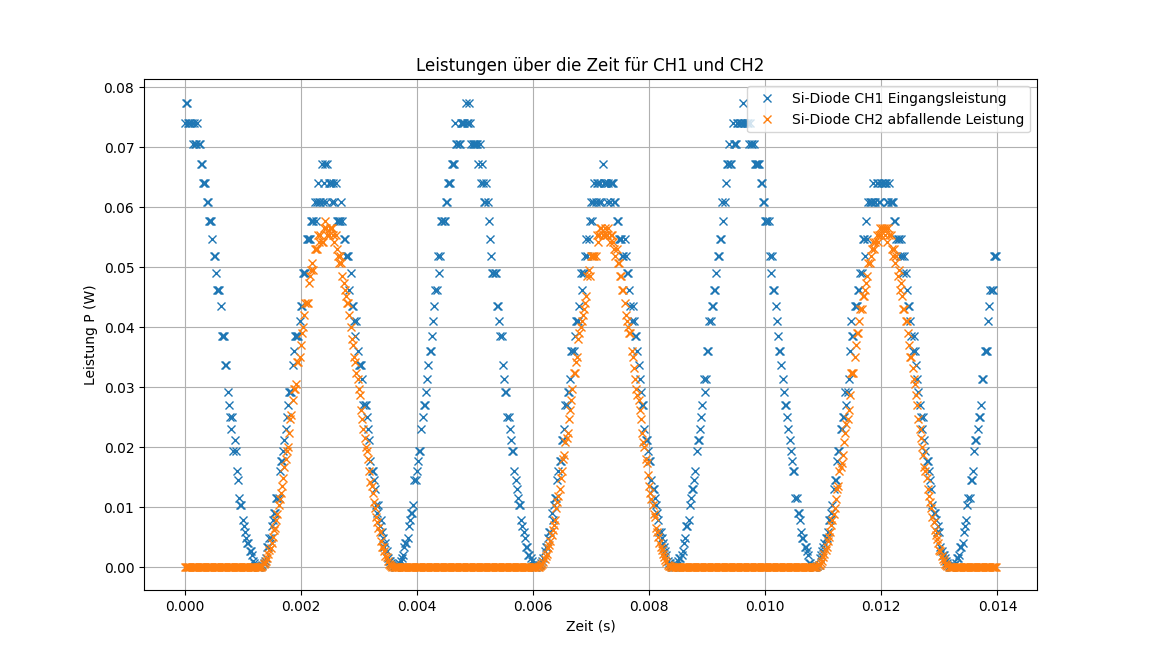
\includegraphics[width=0.9\textwidth]{Leistungen_SiDiode.png}}
	\caption{Eingangsleistung, sowie abfallende Leistung über die Silizium-Diode.}
	\label{fig:PSi}
\end{figure}
\begin{figure}[H]
	\centering{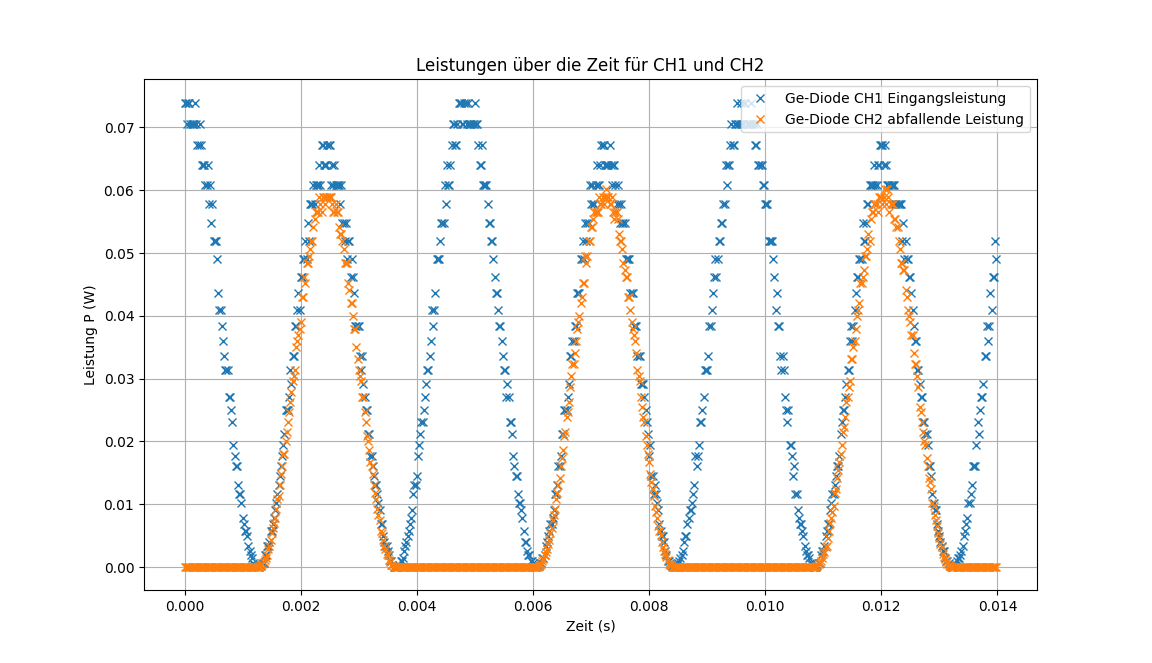
\includegraphics[width=0.9\textwidth]{Leistungen_GeDiode.png}}
	\caption{Eingangsleistung, sowie abfallende Leistung über die Germanium-Diode.}
	\label{fig:PGe}
\end{figure}
\begin{figure}[H]
	\centering{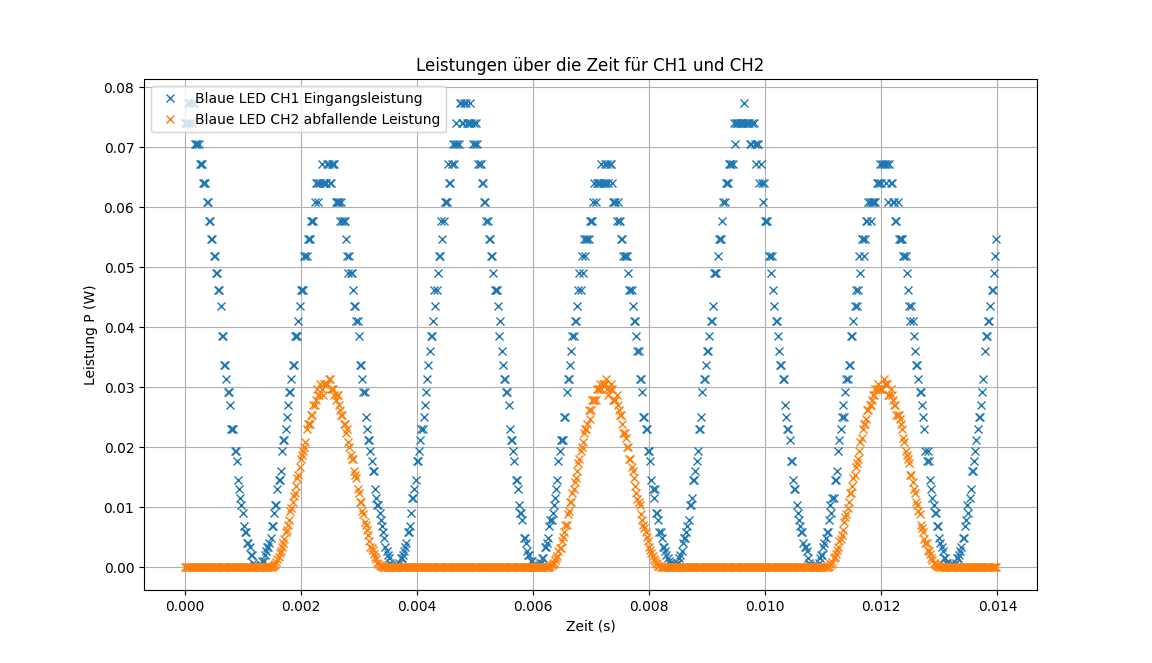
\includegraphics[width=0.9\textwidth]{Leistungen_blaueLED.png}}
	\caption{Eingangsleistung, sowie abfallende Leistung über die blaue LED.}
	\label{fig:PBl}
\end{figure}
\begin{figure}[H]
	\centering{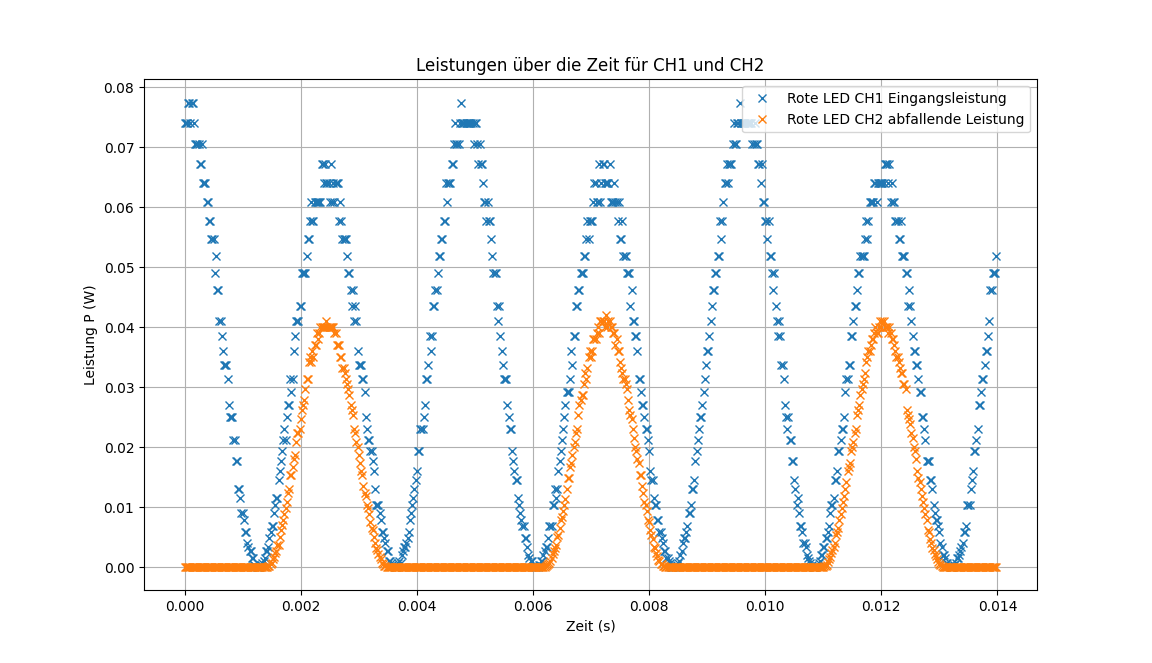
\includegraphics[width=0.9\textwidth]{Leistungen_roteLED.png}}
	\caption{Eingangsleistung, sowie abfallende Leistung über die rote LED.}
	\label{fig:PRo}
\end{figure}

Dabei fällt auf, dass die abfallenden Leistungen bei den LEDs deutlich niedriger sind, als bei den anderen beiden Dioden. Es ist zu beachten, dass die aufgetragenen abgefallenen Leistungen am Widerstand \(R_4\) gemessen wurden, weshalb der Rückschluss sein muss, dass an den beiden LEDs mehr Leistung als an den anderen beiden Dioden abfällt. Dies ist darauf zurückzuführen, dass die LEDs Leistung in Form von Licht abstrahlen.

\section{Zusammenfassung}

Zuerst wurden die Kennlinien von einer Silizium- und einer Germanium-Diode gemessen. Anschließend wurde die Änderung der Leitfähigkeit nach erwärmen auf Körpertemperatur untersucht und die prozentualen Änderungen konnte auf \qty{-4}{\percent} für die Silizium-Diode und \qty{-8}{\percent} für die Germanium-Diode quantifiziert werden.

Es wurden die Sperrkennlinien der Silizium- und Germanium-Diode, sowie die Kennlinie einer Z-Diode und einer roten und einer blauen LED aufgezeichnet. Die unterschiedlichen Schwellspannungen der LEDs wurden aufgrund ihrer Wellenlägen berechnet und konnten die experimentell bestimmten Werte stützen.

Schließlich wurden die abgefallenen Leistungen für alle Dioden graphisch dargestellt und verglichen.

\begin{thebibliography}{999}
	\bibitem{Quelle} Versuchsanleitung zu \emph{E24 -- Halbleiterdioden} (Abgerufen am 29.09.2025).
	Online verfügbar unter: \url{https://www3.physik.uni-stuttgart.de/studium/praktika/ap/pdf_dateien/E24.pdf}
\end{thebibliography}

%\printbibliography
\section{Anhang}

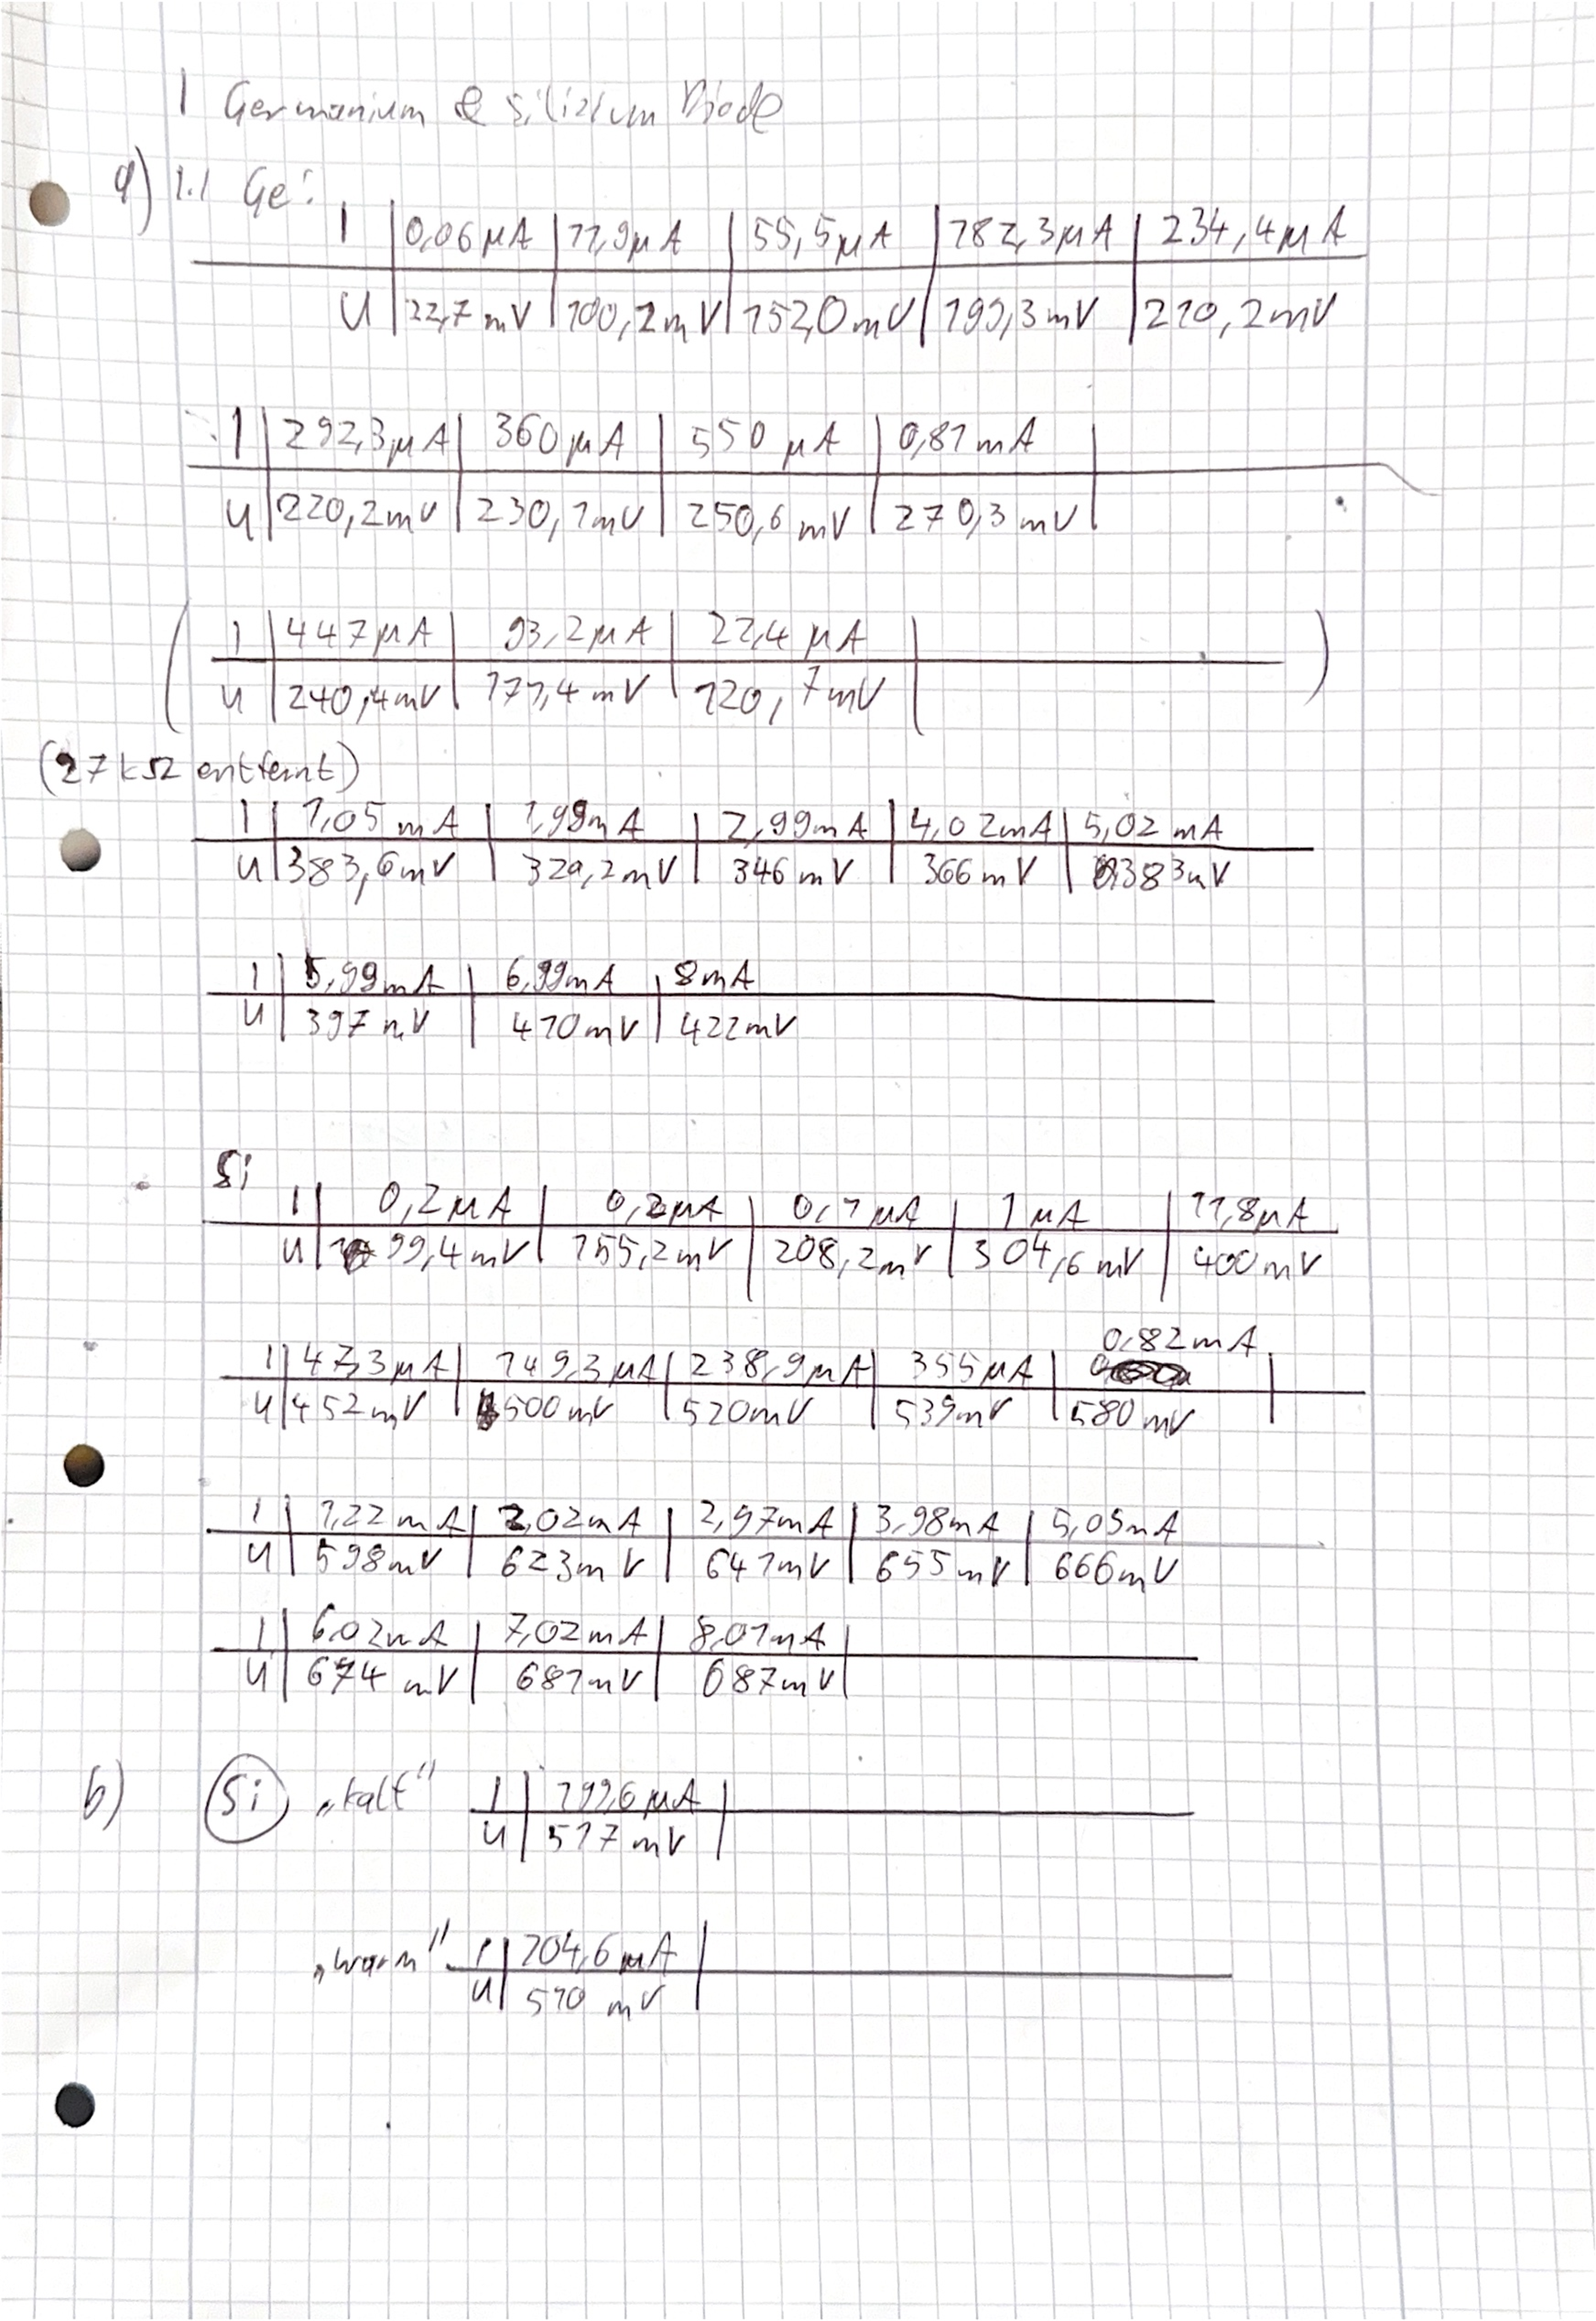
\includepdf[pages=-]{MessprotDioden.pdf}

\end{document}